\part{Results and Discussion}
\label{Chap:Results}

\chapter{Introduction to Results and Discussion}
In this chapter we will present our results for this project and discuss their significance and shortcomings in the context of what we have learned through both our research and our review of the relevant literature. We will begin by looking at the correlations between different variables such as the total sea ice in Antarctica and temperature at gridpoints around the globe. Our hope here is that we similarities in the patterns of correlations which we can associate with different atmospheric or oceanic circulations such as the IPO, ENSO, or the PDO. We then will attempt to quantify the impact on these signals on the amount of sea ice in Antarctica.

\chapter{Correlations}
As our first step in exploring the relationship between sea ice in Antarctica and oceanic and atmospheric weather patterns, we look at correlations between the concentrations of ice in Antarctica both locally and globally over a variety of time scales. 

By looking at the direct correlation at each gridpoint in our dataset between sea ice and different variables we can build up an understanding of what is directly important to the way the ice melts and refreezes each year.

By expanding the scope of this search and looking at the correlation between the amount of ice in Antarctica and global measurements or reanalysis of different variables, we hope to identify what known and unknown circulations impact the behaviour of ice in Antarctica on a global scale.

One thing we noted as we looked through literature on this topic was a tendency of papers to focus in on specific events and follow a chain of causation locally in a short time frame. We hope to investigate the regularity of these events by looking at weather patterns which have been highlighted to see if the phases we see are consistent with particular patterns of ice over a larger number of events throughout our dataset. The correlations we are calculating are our first step in this direction.
\newpage
\section{Local Air Temperature and SIC Correlations}
Firstly we are interested in looking at local effects on the behaviour of sea ice. We do this by taking the correlation between SIC values from the NSIDC dataset and 2m temperature reanalysis values for each gridpoint we have in our dataset. Because the datasets are on different grids, the temperature data has been interpolated to the same grid as the sea ice dataset here.
\begin{figure}[H]
    \centering
    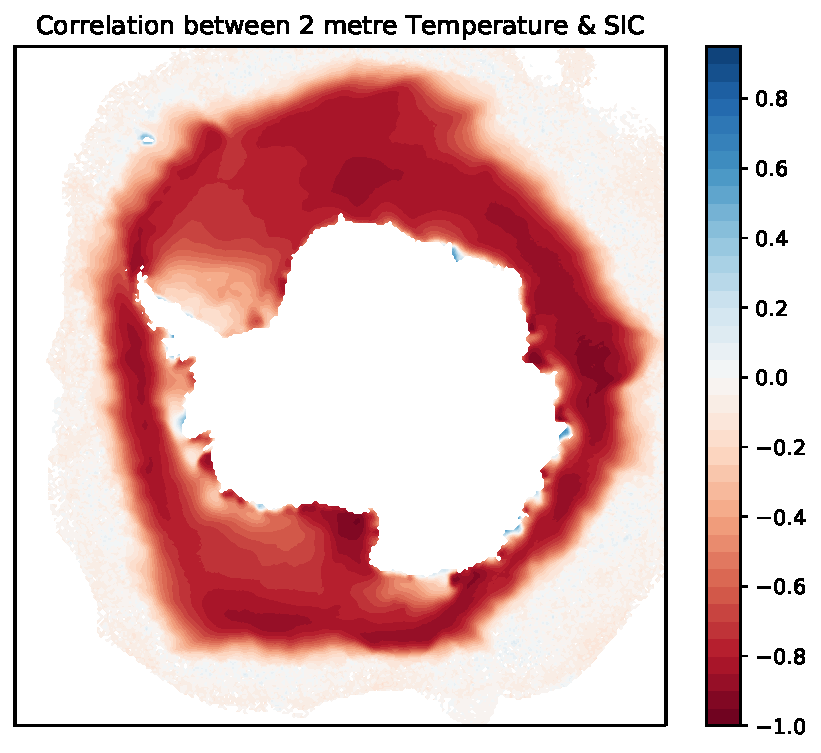
\includegraphics{Images/tempcorrwithsic.pdf}
    \caption{Correlation between temperature at 2m with sea ice concentration.}
    \label{fig:results:2mtemp_corr_with_sic}
\end{figure}

Above we have the correlation between 2 metre air temperature and sea ice concentration over Antarctica. The result that the temperature is negatively correlated with the concentration of sea ice in Antarctica is hardly surprising. Higher temperatures will be associated in the melting of ice. This both intuitively makes sense and is supported by the first law of thermodynamics (Conservation of energy). The main feature of interest in this plot is the regions which are close to the pole and there are lower correlations between 2m-temperature and SIC. It is possible that this is due to low variability in SIC in these regions over the entirety of each year.

\newpage
\section{Correlations with Sea Ice Extent}
In light of work done by other researchers which looked at global temperature correlated with the total amount of sea ice in Antarctica. \cite{Wang2019Compounding2016, Meehl2019Sustained2016} we carried out this comparison ourselves. Taking the Pearson correlation between the time series of 2m temperature at each gridpoint globally with the time series of total sea ice in Antarctica. \textcolor{red}{I'm not sure of the legitimacy of the above paragraph.}

In computing the correlations with SIE in Antarctica, we would expect the largest signal to come from seasonal variations in the different variables. This means that we are expecting large positive and negative correlations for each variable we are looking at, with spatial structures which should give us some physical understanding of how each variable acts in relation to the amount of sea ice around Antarctica.

% \begin{figure}[H]
%     \centering
%     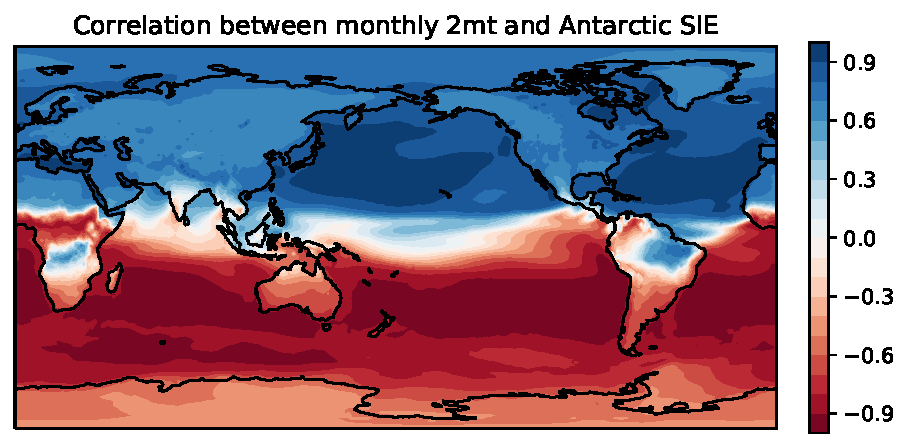
\includegraphics[width=\textwidth]{Images/global_correlation_m2mt_sie.pdf}
%     \caption{Correlation between monthly averaged 2m temperature and total SIE in Antarctica.}
%     \label{fig:my_label}
% \end{figure}

% I haven't done any preprocessing with this data so far. I believe the papers looked at some kind of anomaly in the amount of sea ice, as such I will look into doing something similar next week.
% What we see here however is good as we see a positive correlation in the northern hemisphere and a negative correlation in the southern hemisphere.

% \begin{figure}[H]
%     \centering
%     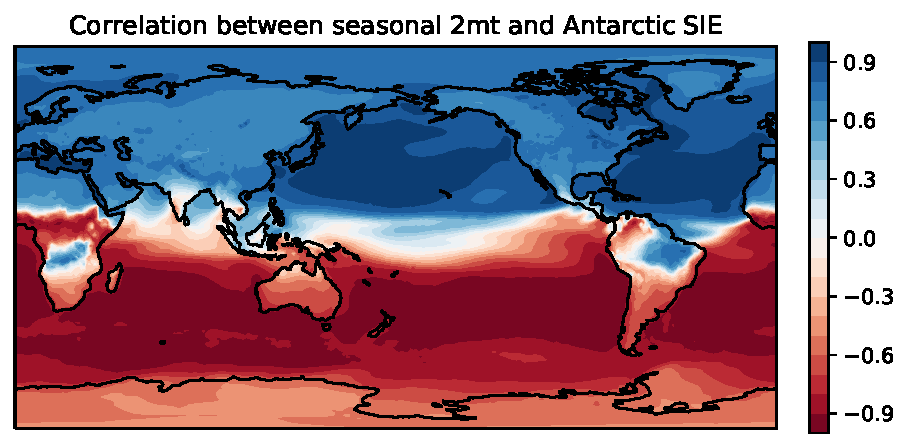
\includegraphics[width=\textwidth]{Images/global_correlation_s2mt_sie.pdf}
%     \caption{Correlation between seasonally averaged 2m temperature and total SIE in Antarctica.}
%     \label{fig:my_label}
% \end{figure}
% We note no difference between the monthly and seasonal correlations between the two datasets. This is good as we would not expect to see a large difference.


\begin{figure}[H]
    \centering
    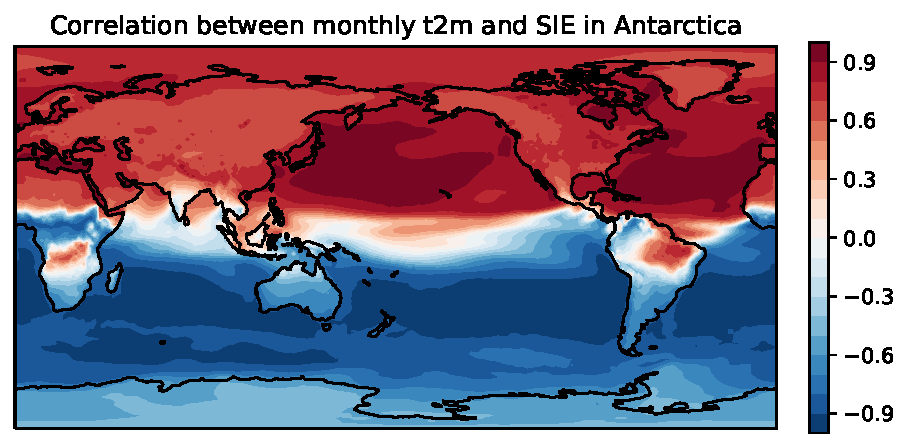
\includegraphics[width=\textwidth]{Images/global_correlation_monthly_t2m_sie.pdf}
    \caption{Correlation between 2m temperature globally and total Sea Ice Extent in Antarctica.}
    \label{fig:temp_sie_corr}
\end{figure}

We note that there is a strong seasonal signal present here. This results in the temperatures in the northern hemisphere being positively correlated with the extent of Antarctic ice. We see a corresponding negative correlation in the southern hemisphere.

We ran the same calculation also for pressure and wind speeds. The results of which are included below.
\begin{figure}[H]
    \centering
    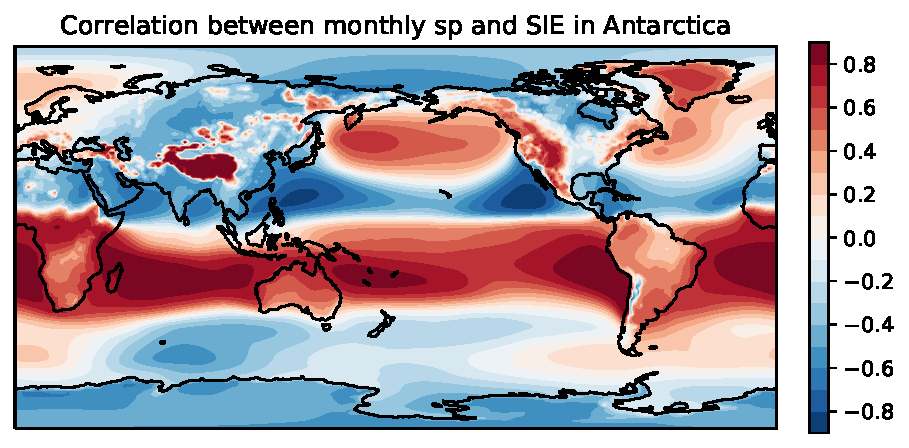
\includegraphics[width=\textwidth]{Images/global_correlation_monthly_sp_sie.pdf}
    \caption{Correlation between surface pressure globally and total Sea Ice Extent in Antarctica.}
    \label{fig:sp_sie_corr}
\end{figure}
We note that the pressure seems to be broken up longitudinally, with a negative correlation near the sea ice followed by a strong positive correlation in the tropics, another negative correlation and then a positive correlation. \textcolor{red}{Possibly because of atmospheric structure? or SAM? Explore.} Also of note is the discrepancies over land in the northern Hemisphere. \textcolor{red}{Maybe Explore?}


\begin{figure}[H]
    \centering
    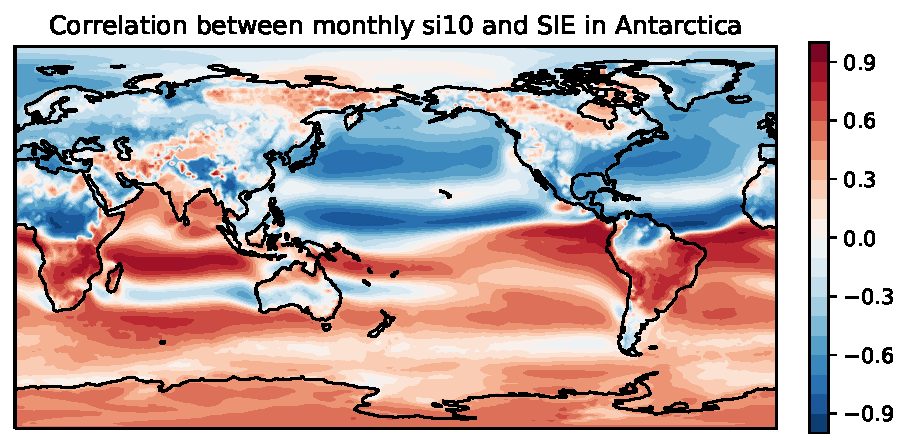
\includegraphics[width=\textwidth]{Images/global_correlation_monthly_si10_sie.pdf}
    \caption{Correlation between 10m wind speed globally and total Sea Ice Extent in Antarctica.}
    \label{fig:si10_sie_corr}
\end{figure}

The total wind speed seems generally split similarly to the temperature correlations, broken up into the northern and southern hemispheres. With generally positive correlations in the southern hemisphere and negative correlations in the northern hemisphere. This indicates potentially a strong seasonal signal which we can explore further by looking at the correlations between SIE and the u and v wind components.

\begin{figure}[H]
    \centering
    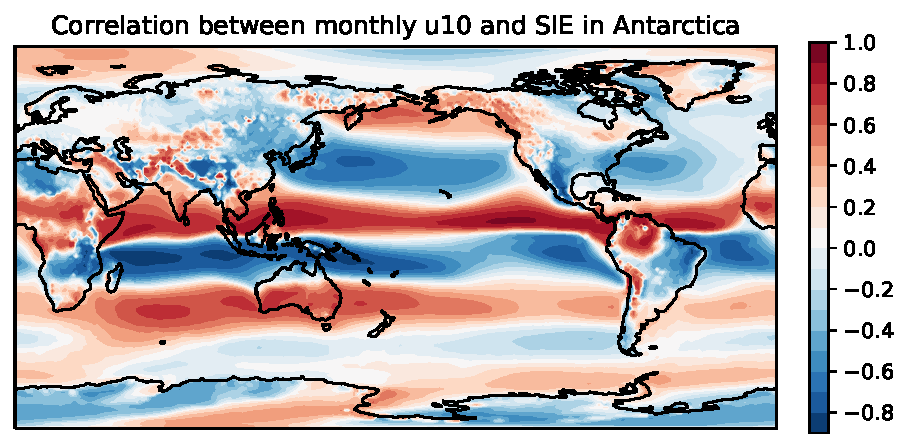
\includegraphics[width=\textwidth]{Images/global_correlation_monthly_u10_sie.pdf}
    \caption{Correlation between u component 10m wind speed globally and total Sea Ice Extent in Antarctica.}
    \label{fig:u10_sie_corr}
\end{figure}

I don't yet have a physical explanation for the bands we see here, but a structure is clearly there and worth discussing. Maybe ENSO?

\begin{figure}[H]
    \centering
    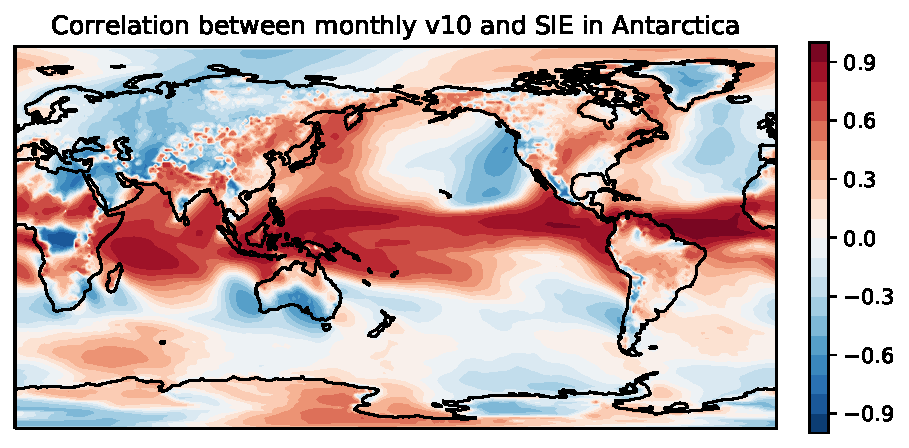
\includegraphics[width=\textwidth]{Images/global_correlation_monthly_v10_sie.pdf}
    \caption{Correlation between v component 10m wind speed globally and total Sea Ice Extent in Antarctica.}
    \label{fig:v10_sie_corr}
\end{figure}

I don't yet have a physical explanation for the bands we see here, but a structure is clearly there and worth discussing.

As expected the largest signal we are seeing in most of these plots is a seasonal one. This makes sense as the seasons are some of the largest climate drivers in the atmosphere and ocean.
\newpage
\section{Anomalous Sea Ice Extent correlations}
We are interested in more complex patterns and relations than the seasonal patterns seen in the section above. As such, we ran the same calculations as before on the anomalies for each time series we have. This was done by removing the mean value for every month from each individual value for that month over the dataset, essentially removing the seasonal component of our data. The results here are presented in the same order as the previous section, starting with 2m temperature.
% As described in the results section, we can calculate the anomaly in our data in multiple ways. For the following results we find the anomaly by removing monthly means from each location, essentially removing the interanual seasonal effect and looking at the more unrelated but perhaps more spatially complex structures in the remaining signal.
% \begin{figure}[H]
%     \begin{subfigure}[b]{\textwidth}
%          \centering
%          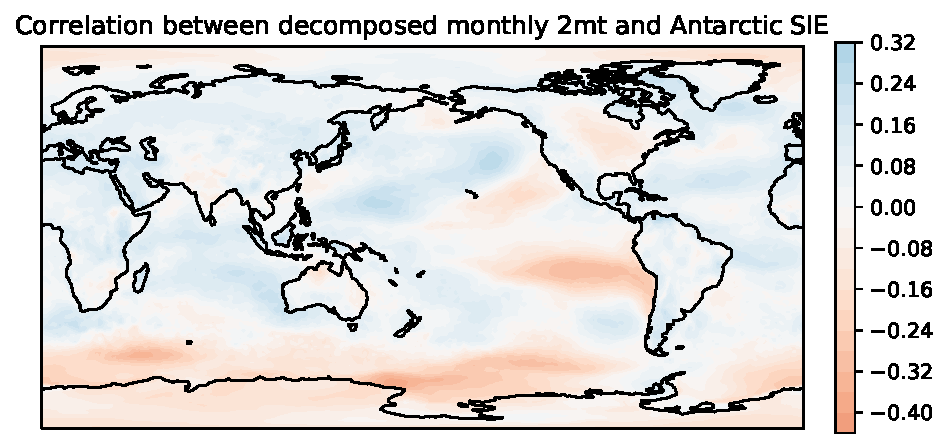
\includegraphics[width=\textwidth]{Images/global_correlation_decomposed_m2mt_sie.pdf}
%         %  \caption{Monthly decomposed 2mt correlated with antarctic SIE}
%          \label{fig:monthly_decomposed_2mt_sie}
%      \end{subfigure}
%      \begin{subfigure}[b]{\textwidth}
%          \centering
%          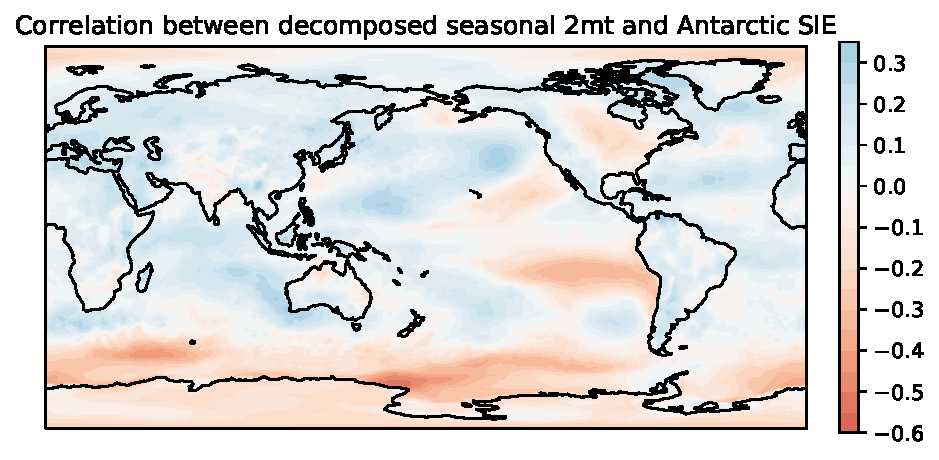
\includegraphics[width=\textwidth]{Images/global_correlation_decomposed_s2mt_sie.pdf}
%         %  \caption{Seasonal decomposed 2mt correlated with antarctic SIE}
%          \label{fig:seasonally_decomposed_2mt_sie}
%      \end{subfigure}
%     \caption{Monthly and seasonal decomposed 2mt correlated with antarctic SIE}
% \end{figure}
% We find little difference between the monthly and seasonal datasets at this point. This is good.
% Additionally, we note that the correlations are low here. This makes sense as there should be no seasonality in the data. Consequently there is also less spatial organisation in the results. The pattern vaguely reminds me of ENSO, so perhaps that is something we could look at moving forward.


\begin{figure}[H]
    \centering
    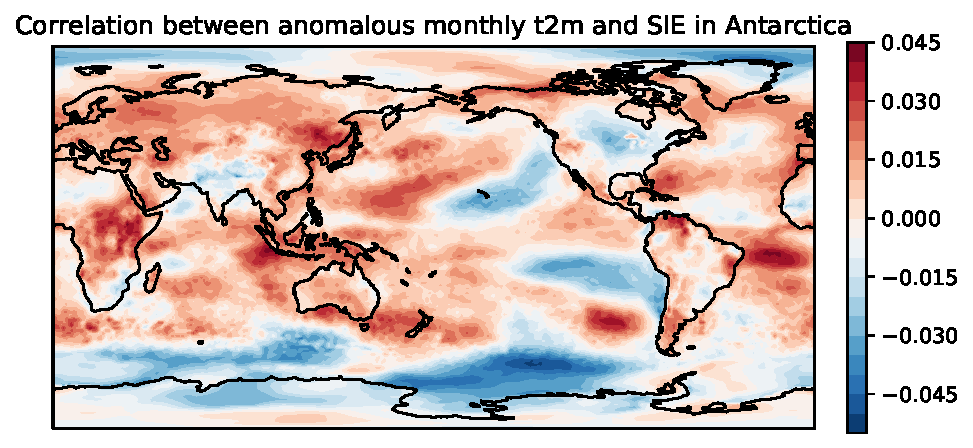
\includegraphics[width=\textwidth]{Images/global_correlation_anomalous_monthly_t2m_sie.pdf}
    \caption{Correlation between anomalous 2m temperature globally and total Sea Ice Extent in Antarctica.}
    \label{fig:t2m_anomalous_sie_corr}
\end{figure}

There is a lot to discuss about this figure, however the thing that stands out the most to me is the IPO pattern. This is something we will potentially want to look at further down the line in our calculations. Next we did the same calculation for surface pressure.

\begin{figure}[H]
    \centering
    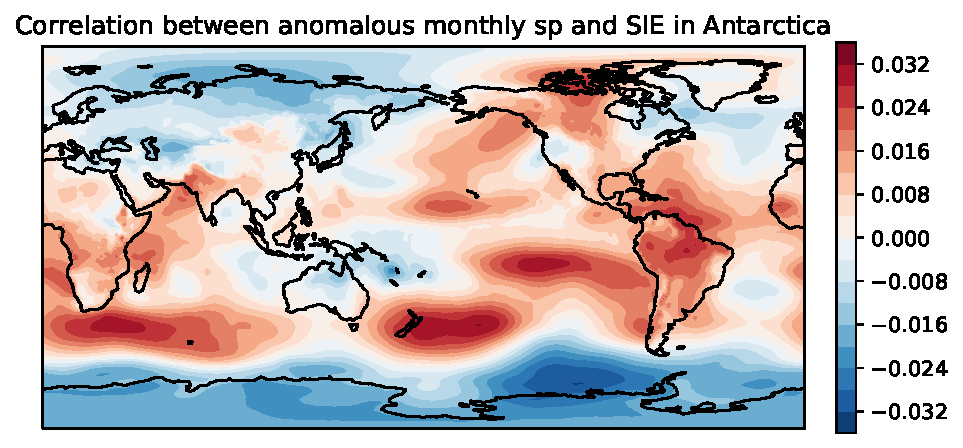
\includegraphics[width=\textwidth]{Images/global_correlation_anomalous_monthly_sp_sie.pdf}
    \caption{Correlation between anomalous surface pressure globally and total Sea Ice Extent in Antarctica.}
    \label{fig:sp_anomalous_sie_corr}
\end{figure}
The first thing to note is how large the signals are for this plot spatially. This is possibly due to how the reanalysis was done or could be showing us something deeper about our climate. I am not entirely sure at this point. Below are the results for the wind correlations.

\begin{figure}[H]
    \centering
    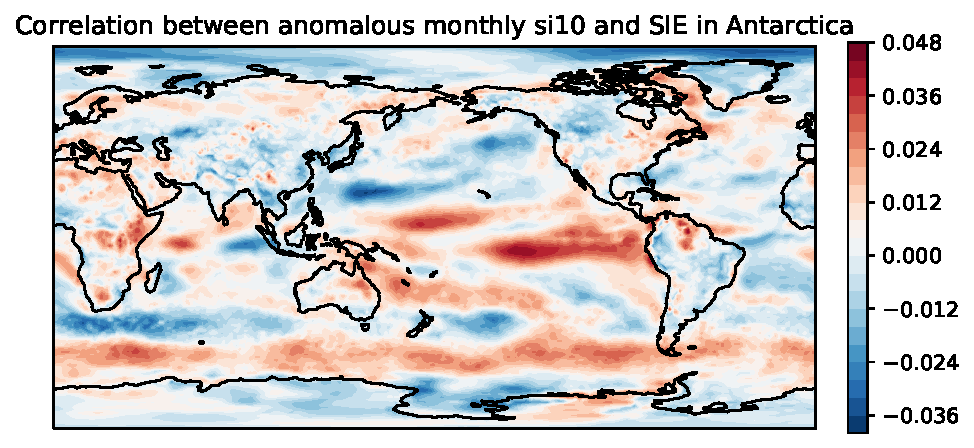
\includegraphics[width=\textwidth]{Images/global_correlation_anomalous_monthly_si10_sie.pdf}
    \caption{Correlation between anomalous 10m wind speed globally and total Sea Ice Extent in Antarctica.}
    \label{fig:si10_anomalous_sie_corr}
\end{figure}

For the total wind speed, the signal which stands out the most looks remarkably like ENSO, this is something we will want to look at further as we continue our analysis.

\begin{figure}[H]
    \centering
    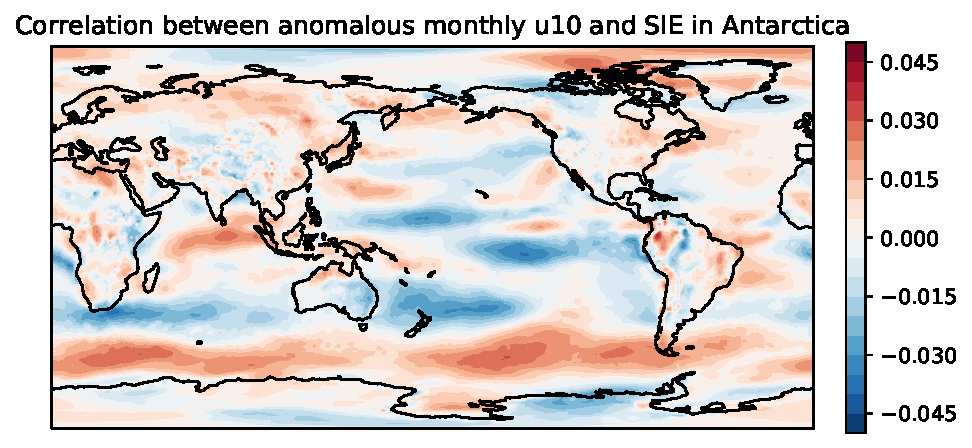
\includegraphics[width=\textwidth]{Images/global_correlation_anomalous_monthly_u10_sie.pdf}
    \caption{Correlation between anomalous u component 10m wind speed globally and total Sea Ice Extent in Antarctica.}
    \label{fig:u10_anomalous_sie_corr}
\end{figure}

For the u component wind, the signal we see could be related to ENSO but it is weaker and less spatially coherent so we cannot be totally sure.

\begin{figure}[H]
    \centering
    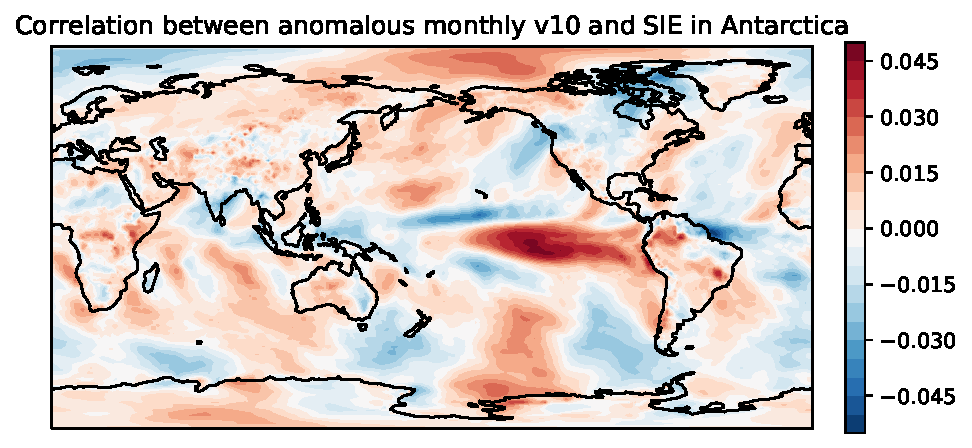
\includegraphics[width=\textwidth]{Images/global_correlation_anomalous_monthly_v10_sie.pdf}
    \caption{Correlation between anomalous v component 10m wind speed globally and total Sea Ice Extent in Antarctica.}
    \label{fig:v10_anomalous_sie_corr}
\end{figure}

For the v component of the wind we see a signal which looks remarkably like ENSO, this is something to look into further.
\newpage
\section{Mean SIC with different indicies}
\begin{table}[H]
\begin{tabular}{@{}rllll@{}}
\toprule
                                      & \textbf{SAM} & \textbf{IPO} & \textbf{DMI} & \textbf{ENSO} \\ \midrule
\textbf{raw monthly}                  & -0.0286      & -0.02356     & 0.149673     & -0.02178      \\
\textbf{raw monthly detrended}        & -0.03614     & -0.01259     & 0.14486      & -0.02917      \\
\textbf{anomalous monthly}            & \textbf{0.153142}     & \textbf{-0.12784}     & 0.112879     & 0.067515      \\
\textbf{anomalous monthly detrended}  & \textbf{0.117848}     & -0.06747     & 0.113995     & 0.02886       \\
\textbf{raw seasonal}                 & -0.04518     & -0.0298      & 0.05791      & -0.01521      \\
\textbf{raw seasonal detrended}       & -0.06096     & -0.0148      & 0.055534     & -0.02615      \\
\textbf{anomalous seasonal}           & \textbf{0.191653}     & -0.14036     & 0.026778     & 0.092851      \\
\textbf{anomalous seasonal detrended} & 0.131356     & -0.06952     & 0.006859     & 0.043756      \\
\textbf{raw annual}                   & 0.270046     & -0.13599     & 0.014287     & 0.115359      \\
\textbf{raw annual detrended}         & 0.13903      & -0.02698     & -0.02919     & 0.028031      \\
\textbf{anomalous annual}             & 0.278939     & -0.16029     & 0.014941     & 0.135027      \\
\textbf{anomalous annual detrended}   & 0.144474     & -0.05059     & -0.03012     & 0.046729      \\ \bottomrule
\end{tabular}
\caption{Correlations between different indices and SIC in Antarctica. Bold values indicate statistical significance i.e. a p-value lower than 0.05.}
\end{table}

% Please add the following required packages to your document preamble:
% \usepackage{booktabs}
\begin{table}[H]
\begin{tabular}{@{}rllll@{}}
\toprule
                                      & \textbf{SAM} & \textbf{IPO} & \textbf{DMI} & \textbf{ENSO} \\ \midrule
\textbf{raw monthly}                  & 0.53     & 0.60     & 0.24     & 0.63      \\
\textbf{raw monthly detrended}        & 0.43     & 0.78     & 0.25     & 0.52      \\
\textbf{anomalous monthly}            & 0.00     & 0.00     & 0.37     & 0.14      \\
\textbf{anomalous monthly detrended}  & 0.00     & 0.14     & 0.37     & 0.52      \\
\textbf{raw seasonal}                 & 0.57     & 0.70     & 0.48     & 0.84      \\
\textbf{raw seasonal detrended}       & 0.44     & 0.85     & 0.50     & 0.74      \\
\textbf{anomalous seasonal}           & 0.01     & 0.07     & 0.74     & 0.24      \\
\textbf{anomalous seasonal detrended} & 0.09     & 0.38     & 0.93     & 0.58      \\
\textbf{raw annual}                   & 0.09     & 0.40     & 0.93     & 0.47      \\
\textbf{raw annual detrended}         & 0.39     & 0.86     & 0.86     & 0.86      \\
\textbf{anomalous annual}             & 0.08     & 0.32     & 0.92     & 0.40      \\
\textbf{anomalous annual detrended}   & 0.37     & 0.75     & 0.85     & 0.77      \\ \bottomrule
\end{tabular}
\caption{p-values for the above correlations.}
\end{table}

\section{Annually averaged results}
For the annually averaged time series, no time-shift was included and there is no difference between the raw and anomalous datasets so we only have two plots, one with the trend and one without.
\begin{figure}[H]
    \centering
    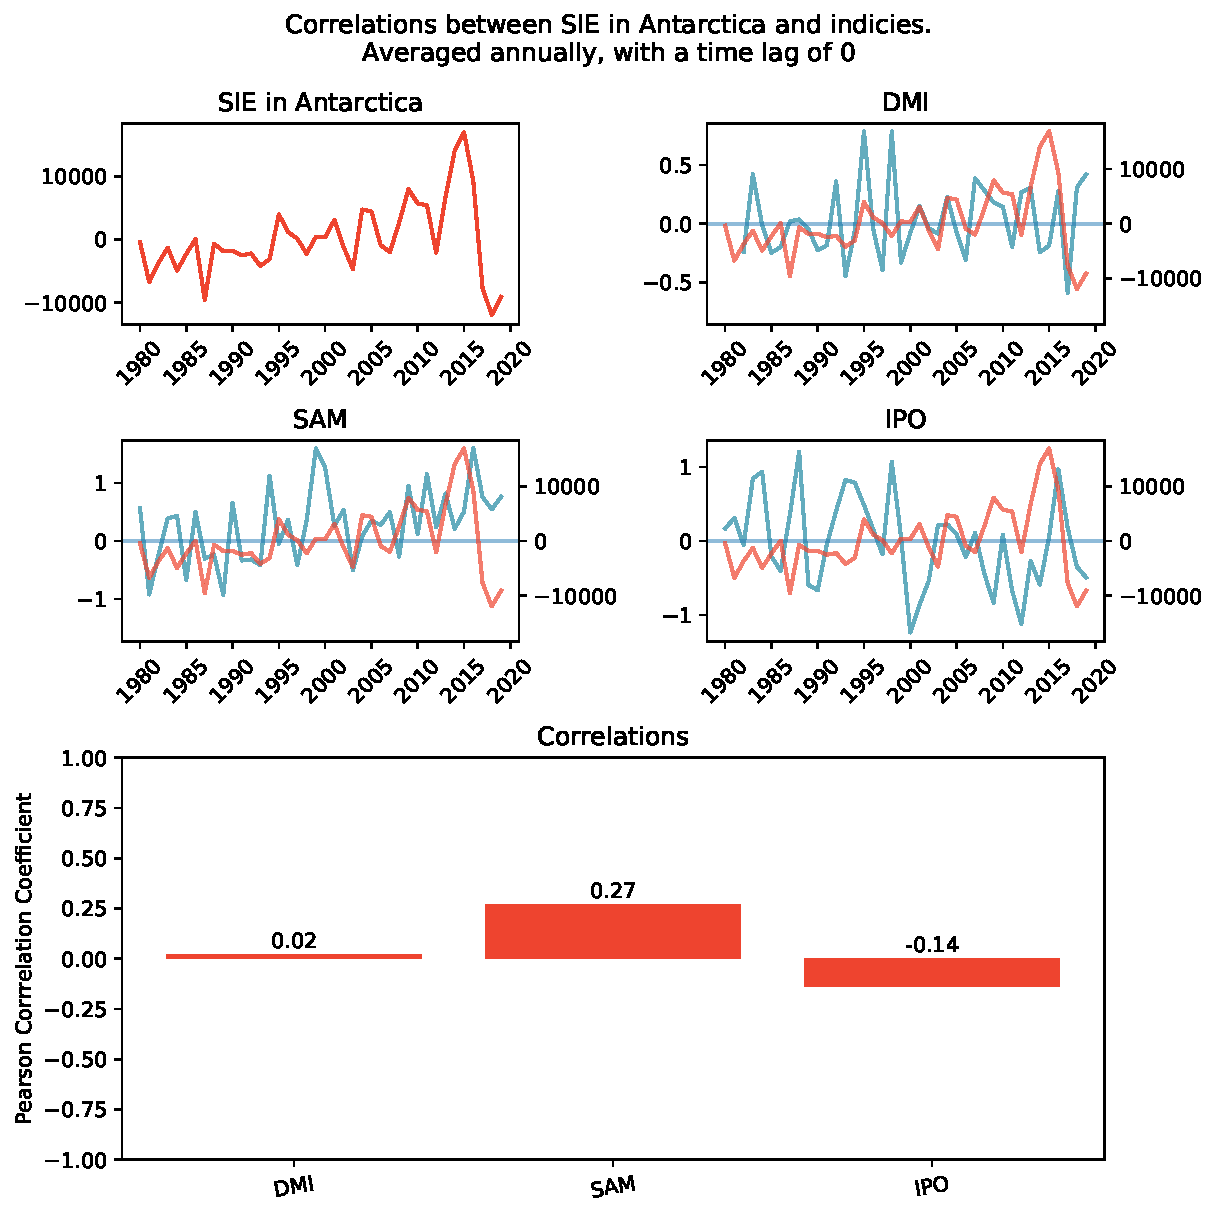
\includegraphics[width=\linewidth]{Images_3.0/correlations/subplots_indicies_annually_0_anomalous.pdf}
    \caption[Correlations between SIE in Antarctica and indices, averaged annually with no time lag.]{Correlations between SIE in Antarctica and indices, averaged annually with no time lag. The first 4 plots are time series of total SIE and the different indices so we can visually gain an understanding regarding the correlations. The bottom plot is a bar plot showing the correlations between SIE and the different indices. Blue bars have a p-value less than 0.05 and are considered statistically significant. Red bars have a p-value larger than 0.05 and are considered statistically insignificant.}
    \label{fig:anual_with_trend}
\end{figure}

\begin{figure}[H]
    \centering
    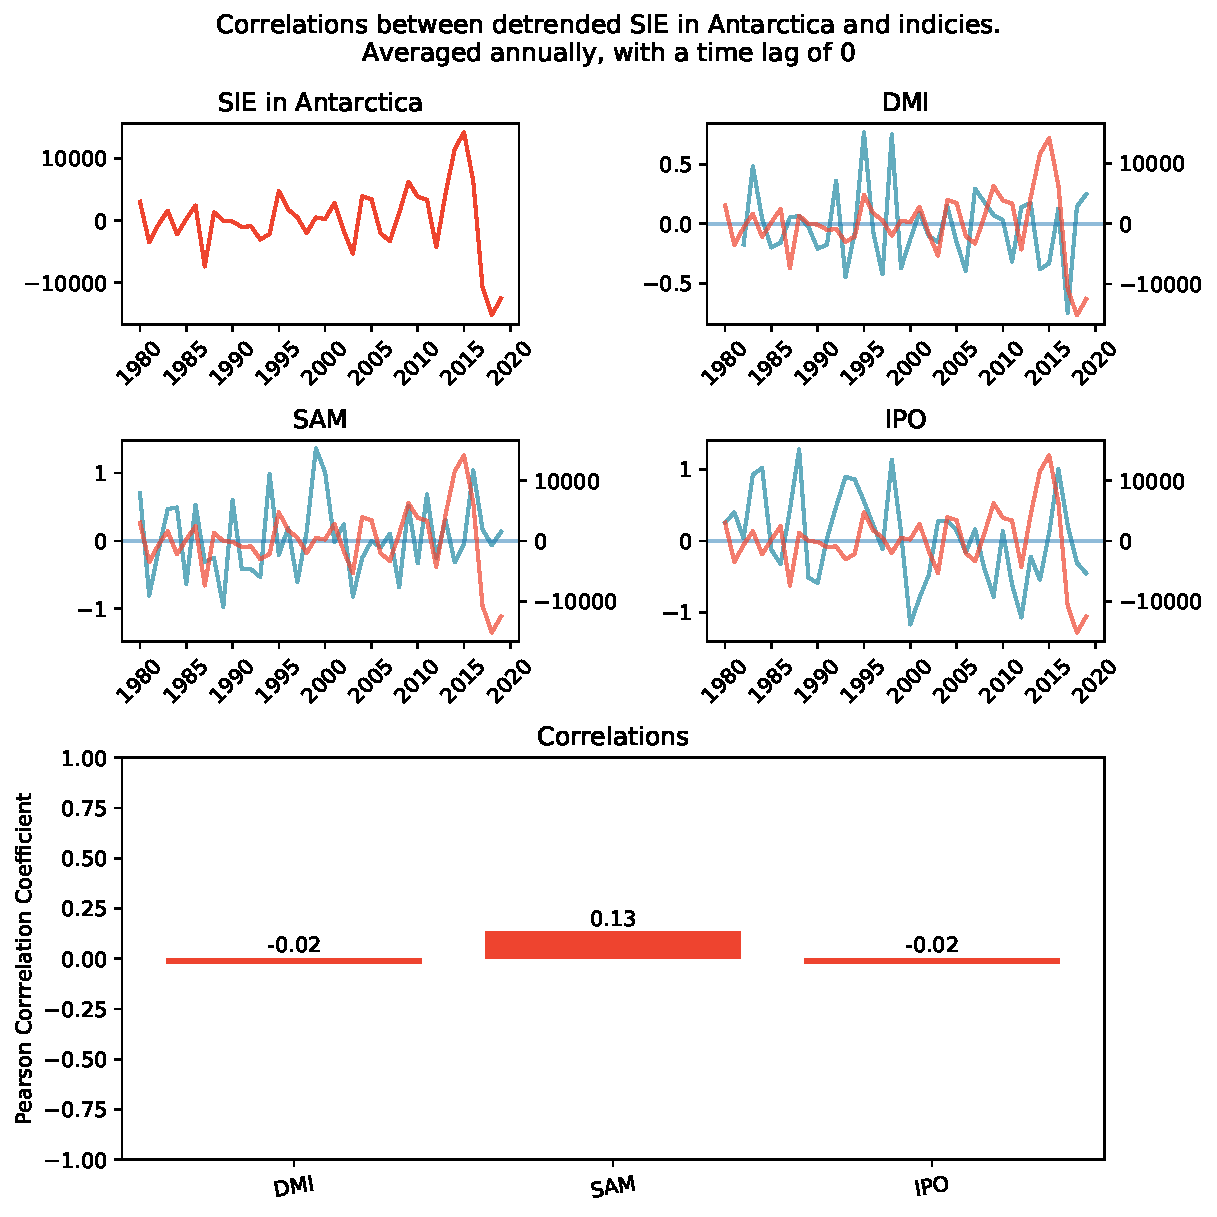
\includegraphics[width=\linewidth]{Images_3.0/correlations/subplots_indicies_annually_0_anomalous_detrended.pdf}
    \caption[Correlations between SIE in Antarctica and indices, averaged annually and detrended with no time lag.]{Correlations between SIE in Antarctica and indices, averaged annually and detrended with no time lag. The first 4 plots are time series of total SIE and the different indices so we can visually gain an understanding regarding the correlations. The bottom plot is a bar plot showing the correlations between SIE and the different indices. Blue bars have a p-value less than 0.05 and are considered statistically significant. Red bars have a p-value larger than 0.05 and are considered statistically insignificant.}
    \label{fig:annual_without_trend}
\end{figure}
Not much can be said from the above figures as all the correlations are insignificant. This could be for a number of reasons, not least because we are only looking at 40 data-points for each time series or that we are considering the behaviour of ice over a large spatial area. Though still statistically insignificant, the correlations are larger for the case where the trend is included.


\section{Monthly averages}

In order to hopefully gain better results, we looked at this with a higher temporal resolution (monthly rather than annually averaged). This has the advantage of picking up higher frequency behaviours, but also is more noisy as a result. Additionally with the higher resolution it makes sense to explore lead-lag relationships between the different variables, this is something we do later in this thesis.


\begin{figure}[H]
    \centering
    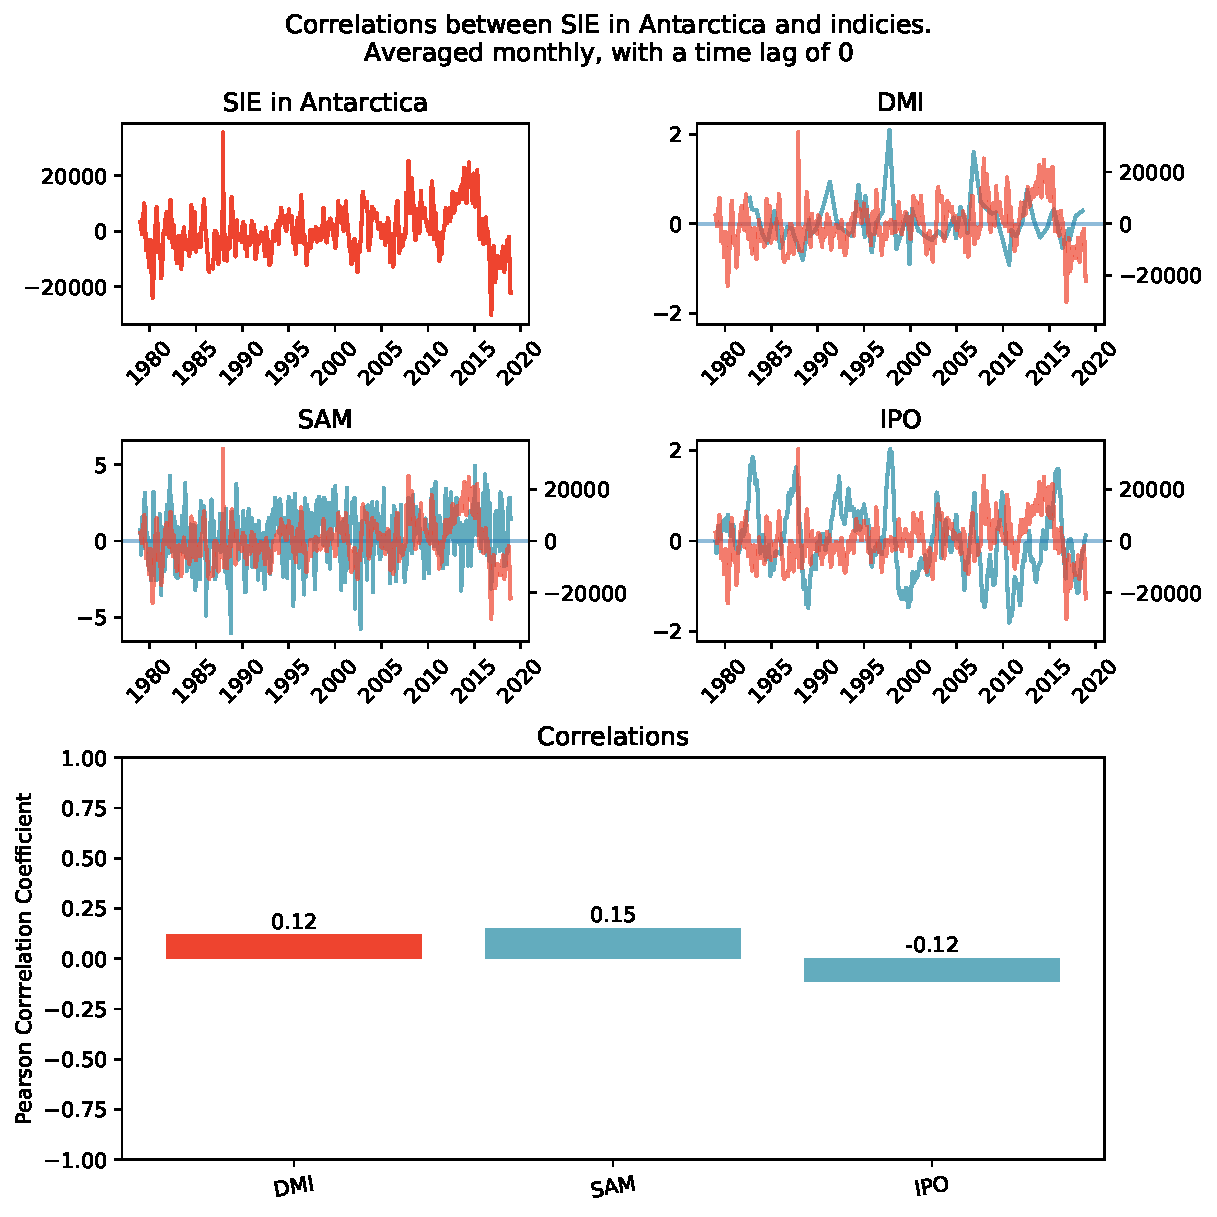
\includegraphics[width = \linewidth]{Images_3.0/correlations/subplots_indicies_monthly_0_anomalous.pdf}
    \caption[Correlations between SIE in Antarctica and indices, averaged monthly with no time lag.]{Correlations between SIE in Antarctica and indices, averaged monthly with no time lag. The first 4 plots are time series of total SIE and the different indices so we can visually gain an understanding regarding the correlations. The bottom plot is a bar plot showing the correlations between SIE and the different indices. Blue bars have a p-value less than 0.05 and are considered statistically significant. Red bars have a p-value larger than 0.05 and are considered statistically insignificant.}
    \label{fig:seasonal_with_trend}
\end{figure}
Immediately, this figure tells us that SAM and IPO both have significant correlations with SIE in Antarctica on a monthly basis. For SAM this is unsurprising as the pattern is defined as changes in wind speeds and pressures at the high southern latitudes close to Antarctica \textcolor{red}{(get proper definition and cite}. For IPO this is also makes some sense as it is a major climate signal over the Pacific. \textcolor{red}{Do other people get the same result?} To help build our understanding of these relationships, let's look at what happens when we detrend the time series.

\begin{figure}[H]
    \centering
    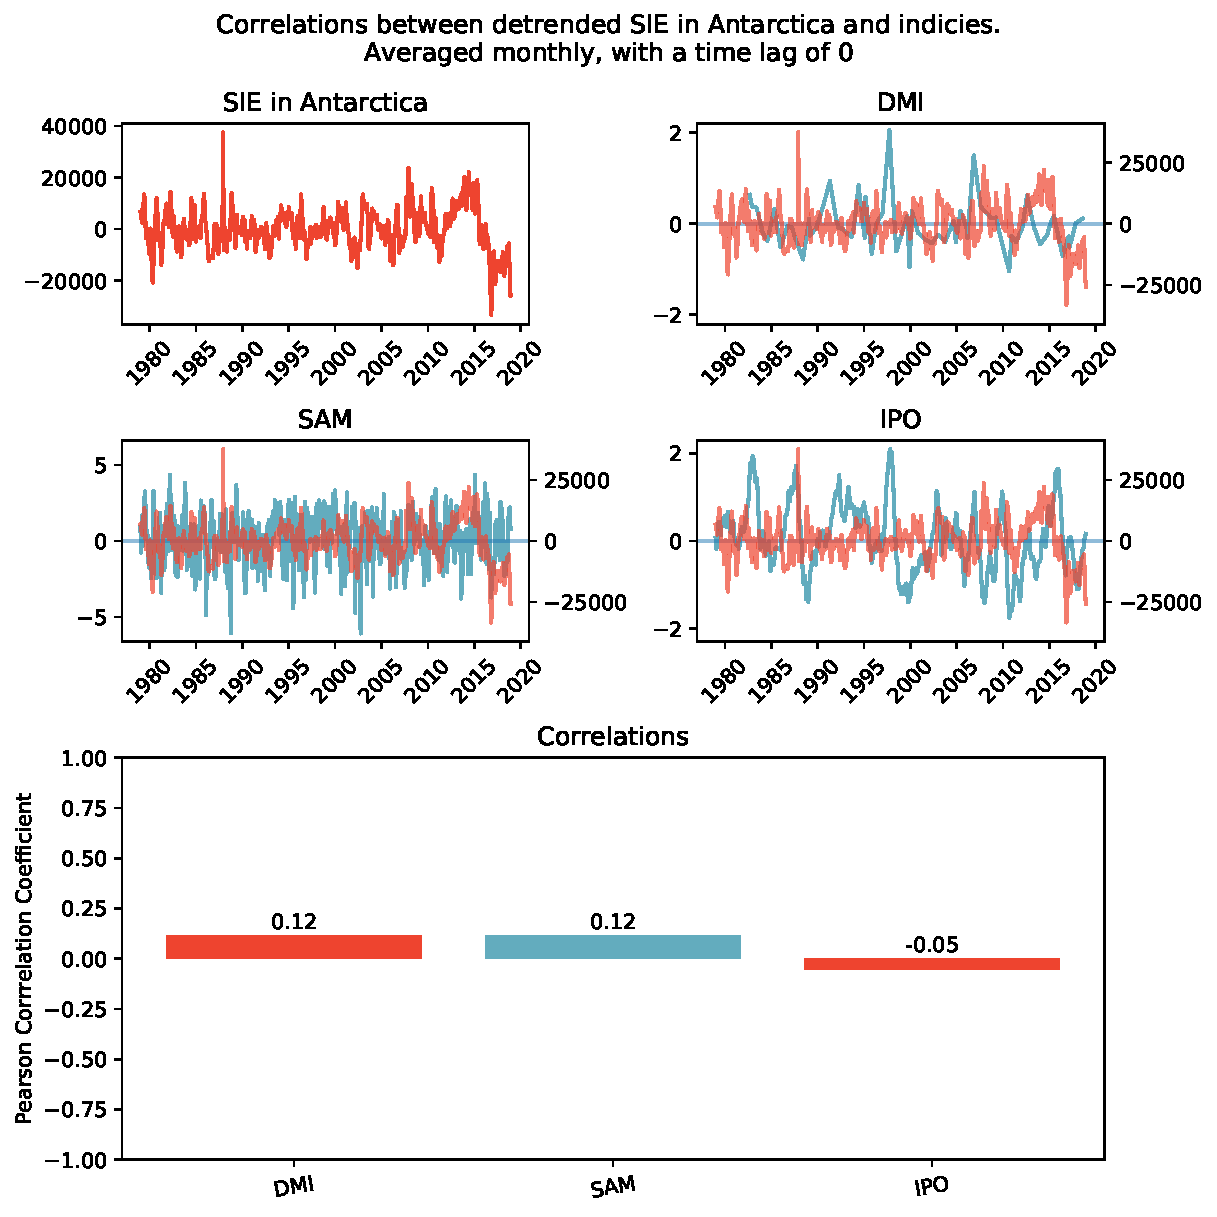
\includegraphics[width = \linewidth]{Images_3.0/correlations/subplots_indicies_monthly_0_anomalous_detrended.pdf}
    \caption[Correlations between SIE in Antarctica and indices, averaged monthly, detrended with no time lag.]{Correlations between SIE in Antarctica and indices, averaged monthly, detrended with no time lag. The first 4 plots are time series of total SIE and the different indices so we can visually gain an understanding regarding the correlations. The bottom plot is a bar plot showing the correlations between SIE and the different indices. Blue bars have a p-value less than 0.05 and are considered statistically significant. Red bars have a p-value larger than 0.05 and are considered statistically insignificant.}
    \label{fig:seasonal_without_trend}
\end{figure}

When we remove the trend the magnitude of the correlations decrease for SAM and IPO, whereas DMI has no change in the magnitude of correlation. The correlation between SAM and SIE in Antarctica remains statistically significant whereas the IPO is no longer significant. 


\section{Lead lag analysis for monthly data}

We can perform some lead-lag analysis on the correlations between the different indices and SIE in Antarctica, to gain some understanding on if there are any delayed signals of significance we need to consider. Because the indices are initially anomalous signals, we only did this for the anomalous sea ice data. In the following plots, a negative time-lag indicates that we are comparing the time-series for sea ice with patterns in each index before that point. A positive time-lag indicates that we are comparing the time-series for sea ice with patterns in each index after that point. The size of the time-lag indicates the length to which the sea ice time series was shifted.
\begin{figure}[H]
    \centering
    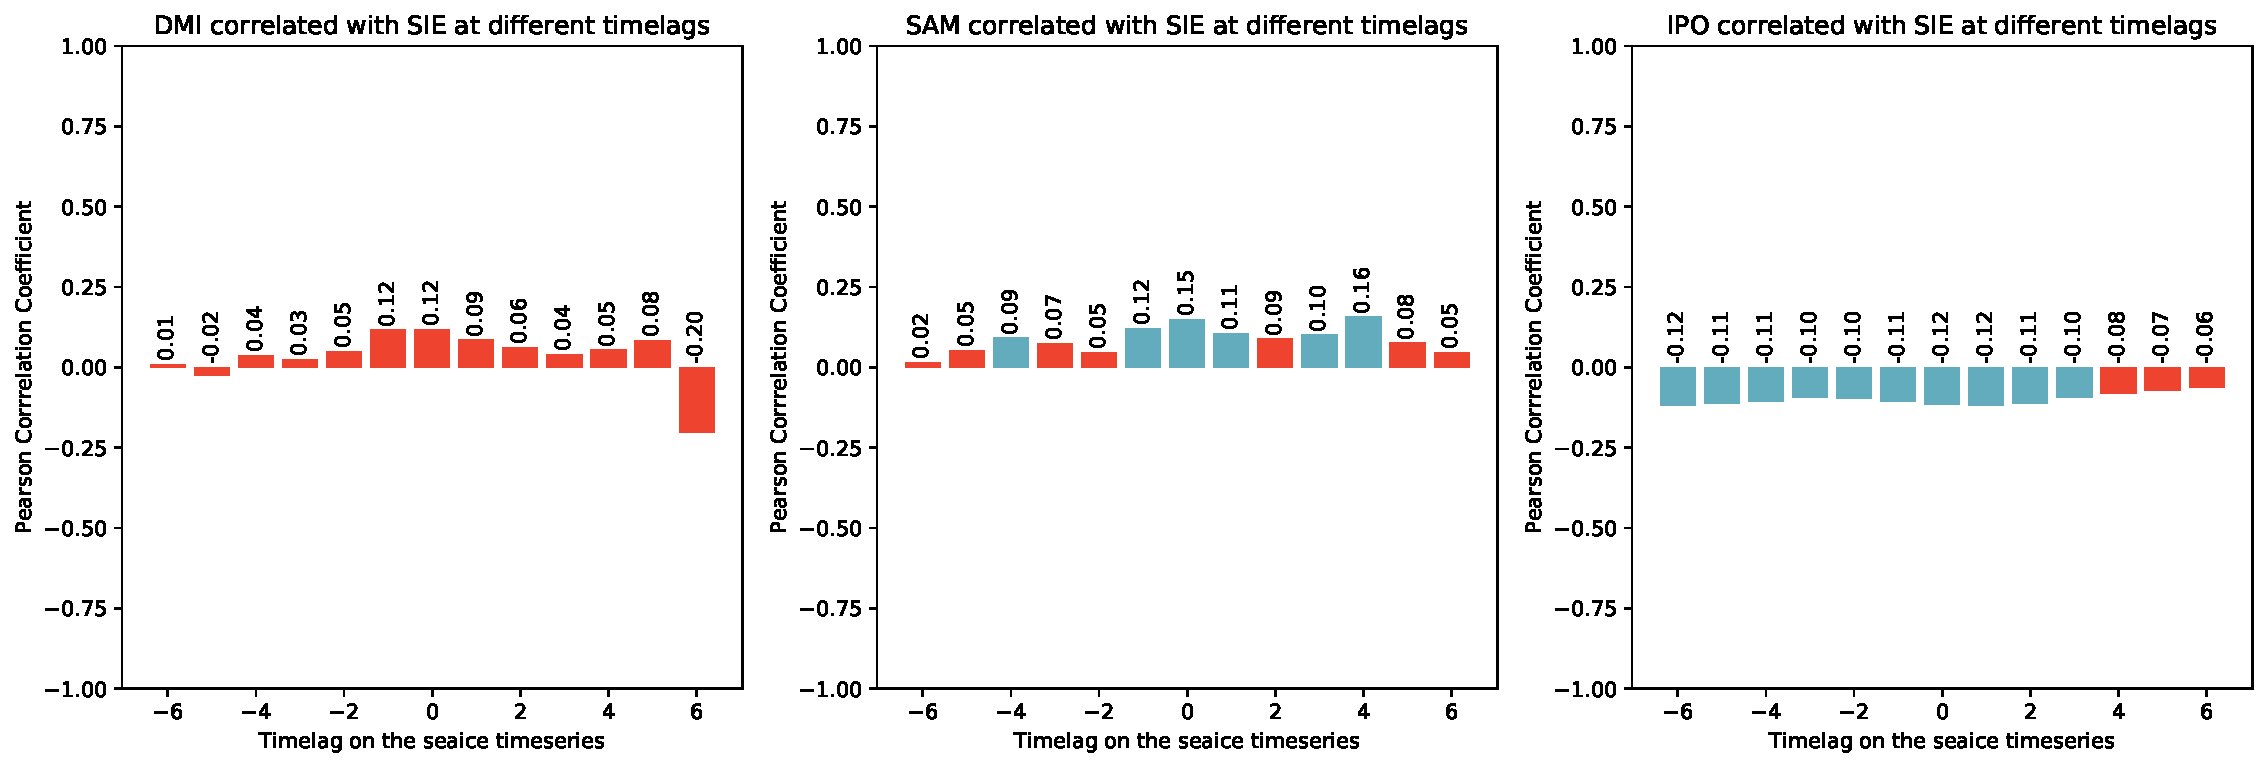
\includegraphics[width = \linewidth]{Images_3.0/correlations/indicies_monthly_anomalous.pdf}
    \caption[Histograms of correlations with different indices at different time-lags with anomalous Antarctic SIE.]{Histograms of correlations with different indices at different time-lags with anomalous Antarctic SIE. A blue bar indicates a statistically significant p-value of less than 0.05. A red bar indicates a statistically insignificant value.}
    \label{fig:leadlag_anomalous}
\end{figure}

DMI has no significant correlation with Antarctic SIE regardless of time-lag. SAM has a significant correlation for time-lags of -1, 0, 1, 3, 4, and 5 months. IPO has significant correlations for any time-lag less than 3 months (including negative time-lags). It's possible that the trend is confusing the signals here so let's see what happens when we remove it.

\begin{figure}[H]
    \centering
    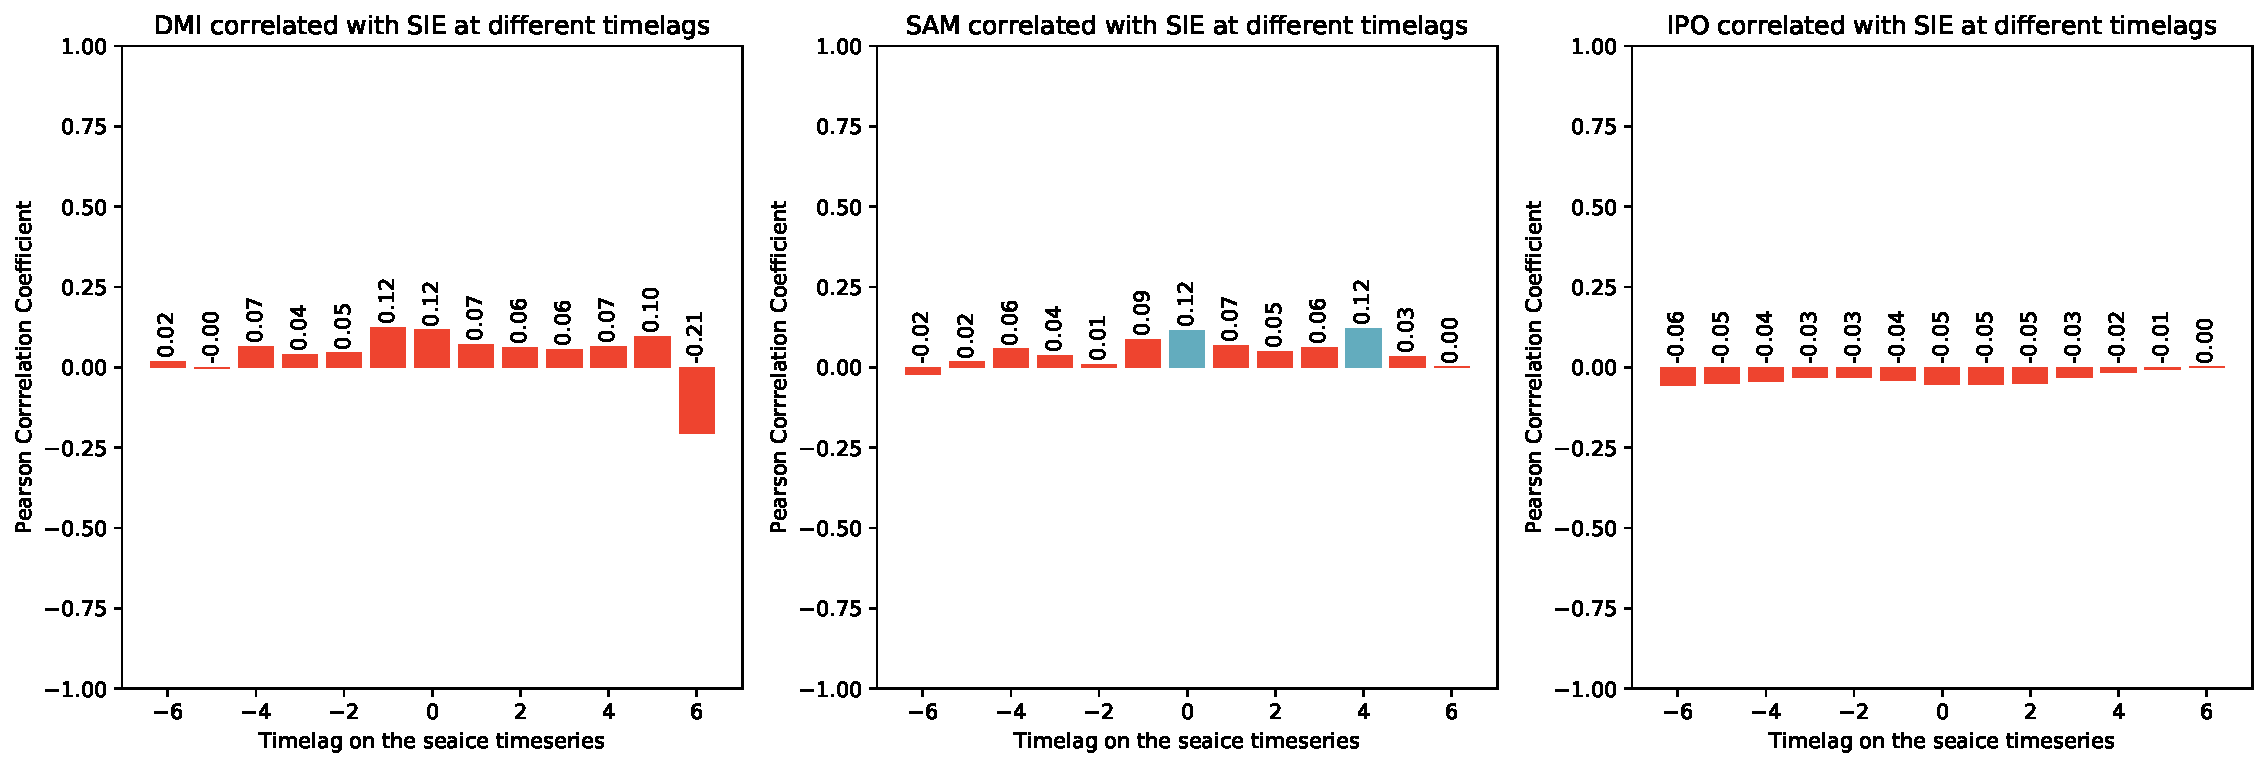
\includegraphics[width = \linewidth]{Images_3.0/correlations/indicies_monthly_anomalous_detrended.pdf}
    \caption[Histograms of correlations with different indices at different time-lags with anomalous and detrended Antarctic SIE.]{Histograms of correlations with different indices at different time-lags with anomalous and detrended Antarctic SIE. A blue bar indicates a statistically significant p-value of less than 0.05. A red bar indicates a statistically insignificant value.}
    \label{fig:leadlag_anomalous_detrended}
\end{figure}

The only significant correlations we observe at this point are the correlations between SAM and Antarctic SIE for time-lags of 0 and 4 months. This indicates that when an event occurs for Antarctic SIE, it is likely that we would observe a related event in the SAM index at the same time and also 4 months later. \textcolor{red}{not sure if I worded this right so let's go with it for now.}\medskip

One problem we have here is that we are not totally able to use the information for the correlations which we have above to inform us regarding how events for the different indexed circulations could potentially impact the behaviour of sea ice we see in Antarctica. For that we want to look at the first time derivative of Antarctic SIE to see if it has behaviours related to these indices.
\newpage
\section{Splitting the data}
Throughout literature surrounding the behaviour of Antarctic SIE, there is a large focus on the overall increase in SIE up to 2014, \cite{Parkinson2019} for instance spends some time discussing this, as does \cite{Yuan2017}. They also go into some detail of the spatial variability. More focus is also put on the large decrease in the SIE from 2014 where we get the record largest amount of SIE to 2016 when we get the record lowest SIE. \cite{Meehl2018}
\newpage


\chapter{Regressions}

Following on from the correlation results shown before it is apparent that there are potential relationships between the different atmospheric circulations and the behaviour in trends and variability of sea ice extent in Antarctica. The next step is to begin to quantify the extent of this relationship by performing a regression analysis. The mechanics of how these figures are produced are described in detail in the method section \textcolor{red}{cross-reference this}. 

For this section we will start by looking at the mean SIE across the entire continent and fit it to a simple linear model which predicts a value of SIE from the values of the different circulations we are looking at. To begin with this is SAM, DMI and IPO, however as our analysis expands, we plan to look at other influential circulations such as ENSO.

Following this we will perform the same analysis on each gridpoint of sea-ice and look at the spatial distribution of this regression. Using it to quantify and investigate the extent to which we can account for variability in SIE to these different indices.

What we are expecting to see is that SAM will have the largest impact on long term trends and DMI and IPO will be more important for describing short term variability.

\newpage
\section{Regression analysis on mean annual SIE}

Before doing any spatial analysis we will take a moment to apply the regression analysis to the mean value of SIE over our time period. The simplest and first step we take is to plot the annual values of SIE against each of the indices we are investigating.
\begin{figure}[H]
    \centering
    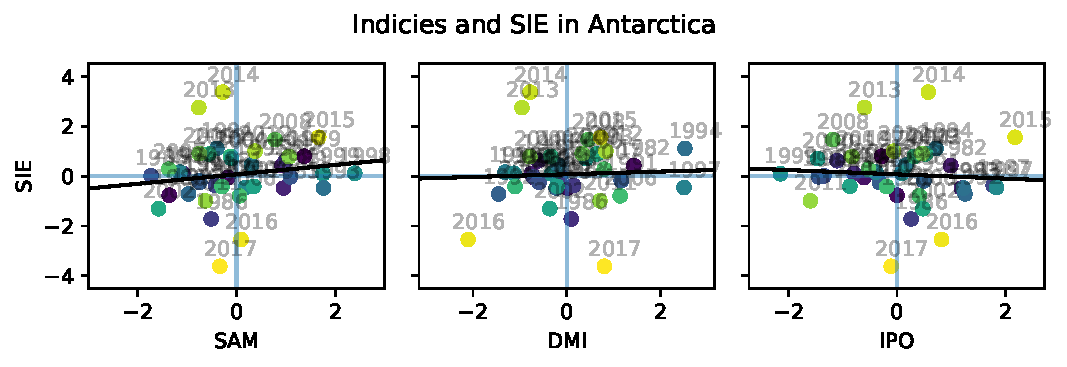
\includegraphics[width=\linewidth]{Images_3.0/regressions/scatter_anomalous_n1_annually_detrended_1979_2018.pdf}
    \caption{Regression of SIC for each of the indices for 1979 to 2018.}
    \label{fig:scatter_anomalous_n1_annually_1979_2018}
\end{figure}
We note that these results are consistent with what we found in the correlation analysis. SAM has a positive relationship with SIE, while DMI has a very weak positive relationship and IPO has a weak negative relationship. This doesn't give us new information, however the consistency indicates that the regression analysis provides somewhat reliable results results. Plotting the same thing for before and after December 2001 when IPO is in negative and positive phases respectively gives the following plots.

\begin{figure}[H]
    \begin{subfigure}{\linewidth}
    \centering
    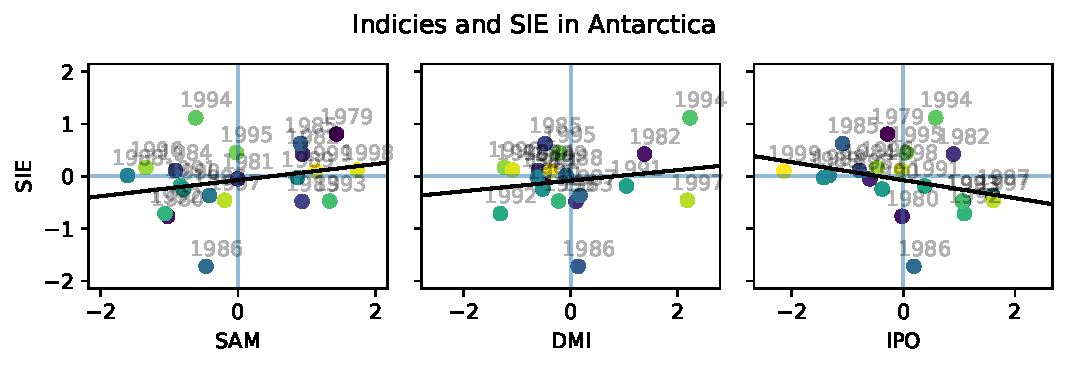
\includegraphics[width=\linewidth]{Images_3.0/regressions/scatter_anomalous_n1_annually_detrended_1979_2000.pdf}
    \caption{Regression of SIC for each of the indices for 1979 to 2000.}
    \label{fig:scatter_anomalous_n1_annually_1979_2000}
    \end{subfigure}
    
    \begin{subfigure}{\linewidth}
    \centering
    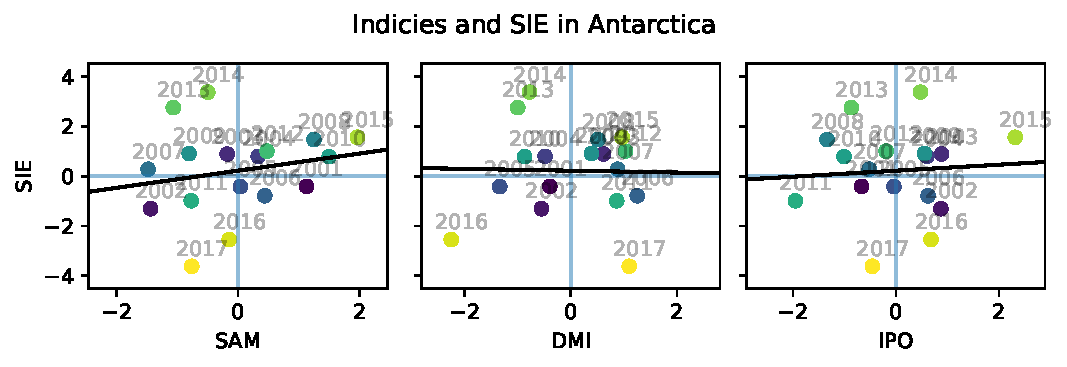
\includegraphics[width=\linewidth]{Images_3.0/regressions/scatter_anomalous_n1_annually_detrended_2001_2018.pdf}
    \caption{Regression of SIC for each of the indices for 2001 to 2018.}
    \label{fig:scatter_anomalous_n1_annually_2001_2018}
    \end{subfigure}
    \caption{Regressions for SIE for the different time periods in our dataset.}
\end{figure}
Here we can see that there is little change for the SAM relationship with SIE whereas the relationship between IPO experiences a significant change, shifting from a negative relationship before 2001 and a positive relationship after 2001. DMI has a positive relationship before 2001 and a weak negative relationship after 2001.

\subsection{Regression analysis on mean monthly SIE}
We have the same plots for the monthly version of the data.
\begin{figure}[H]
    \begin{subfigure}{\linewidth}
    \centering
    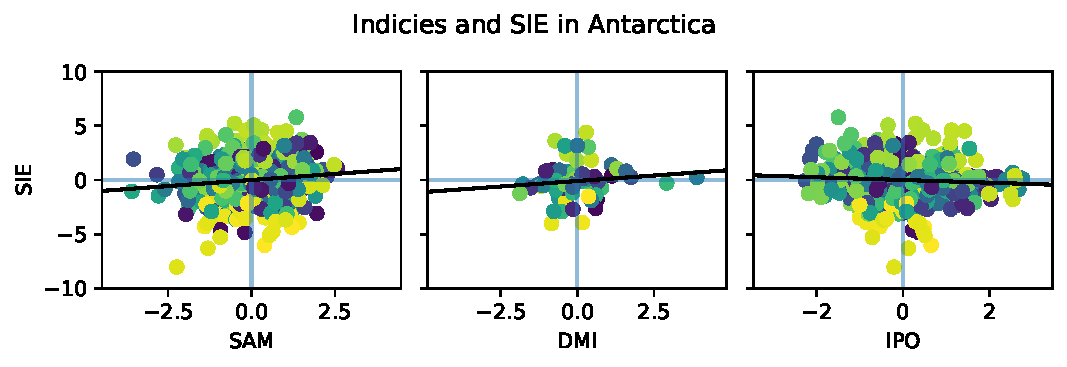
\includegraphics[width=\linewidth]{Images_3.0/regressions/scatter_anomalous_n1_monthly_detrended_1979_2018.pdf}
    \caption{Regression of SIC for each of the indices for 1979 to 2018.}
    \label{fig:scatter_anomalous_n1_annually_1979_2018}
    \end{subfigure}
    
    \begin{subfigure}{\linewidth}
    \centering
    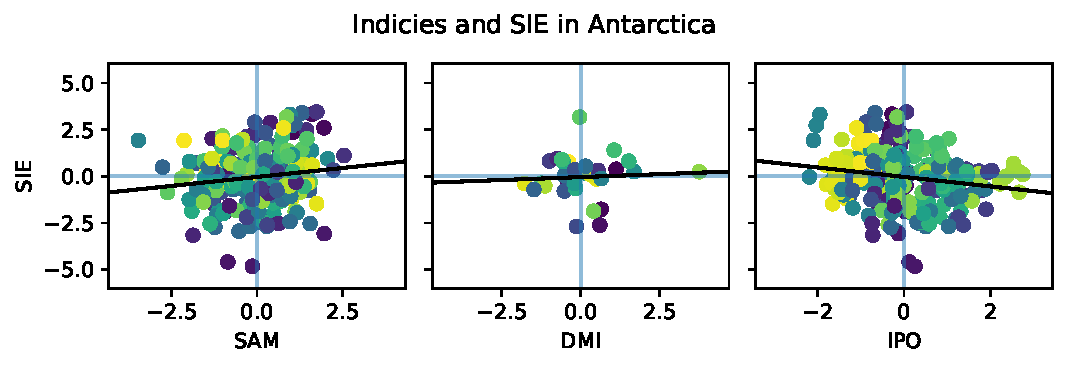
\includegraphics[width=\linewidth]{Images_3.0/regressions/scatter_anomalous_n1_monthly_detrended_1979_2000.pdf}
    \caption{Regression of SIC for each of the indices for 1979 to 2000.}
    \label{fig:scatter_anomalous_n1_annually_1979_2000}
    \end{subfigure}
    
    \begin{subfigure}{\linewidth}
    \centering
    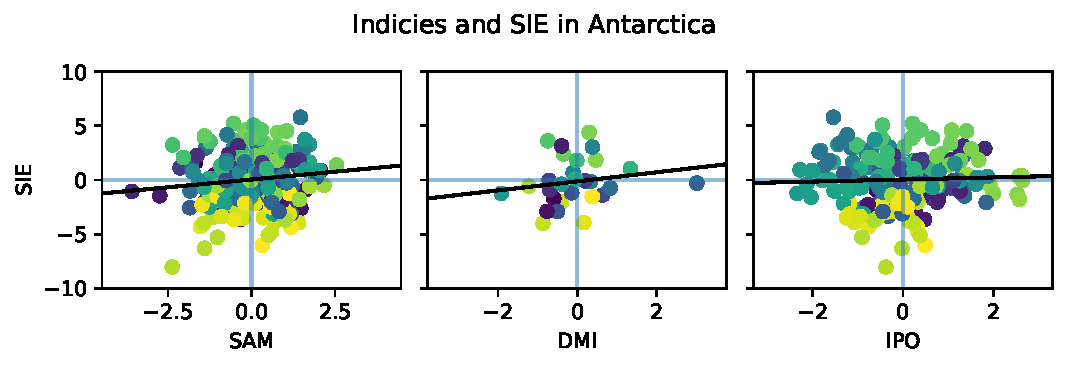
\includegraphics[width=\linewidth]{Images_3.0/regressions/scatter_anomalous_n1_monthly_detrended_2001_2018.pdf}
    \caption{Regression of SIC for each of the indices for 2001 to 2018.}
    \label{fig:scatter_anomalous_n1_annually_2001_2018}
    \end{subfigure}
    \caption[Regressions for SIE for the different time periods in our dataset.]{Regressions for SIE for the different time periods in our dataset. The colour represents years with blue being early years and yellow representing latter years.}
\end{figure}
The main difference in these plots when compared with the annual averages is the relationship between SIE and IPO and DMI after 2001. DMI has a positive relationship for the monthly means whereas it has a negative relationship for the annual means. IPO has a weaker relationship for the monthly means than the annual means.
\section{Applying the regression model}
After doing this initial analysis we can apply the regression analysis using the model:
$$
\text{SIE} = a\times\text{SAM} + b\times\text{DMI} + c \times\text{IPO} + d
$$
We can look at the quality of this fit by plotting this model prediction and the actual SIE time-series against each other.
\begin{figure}[H]
    % \begin{subfigure}{\linewidth}
    \centering
    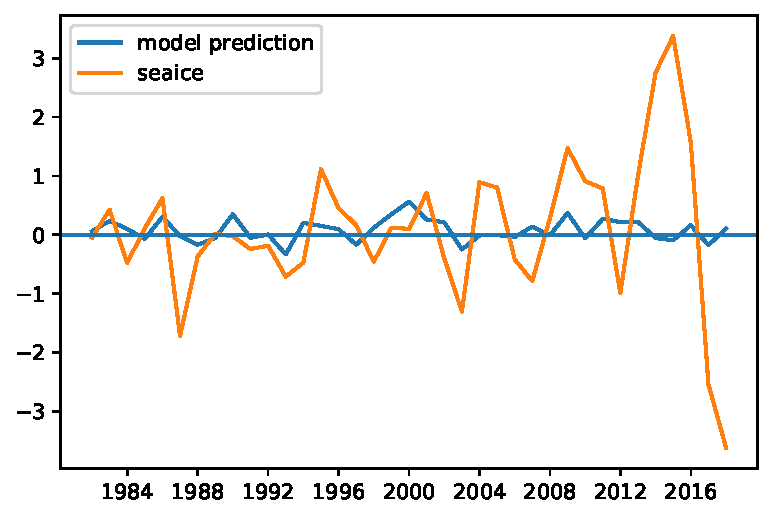
\includegraphics{Images_3.0/regressions/multivariate_model_anomalous_n1_annually_detrended_1979_2018.pdf}
    \caption{Fitted model for SIE detrended and averaged annually from 1979 to 2018.}
    \label{fig:multivariate_model_anomalous_n1_annually_detrended_1979_2018}
    % \end{subfigure}
\end{figure}
This doesn't seem to be a good fitting. This isn't surprising for a number of reasons. Firstly the regressions done on each individual index were each relatively weak and so we don't expect a strong fitting when done in concert. Additionally the system we are looking at is intrinsically complex and probably nonlinear, which leads to a bad fitting with a linear model. Additionally because we are only looking at the mean value for SIE this plot will have lost information because the indices probably affect different spatial regions of SIC in different ways. This is something we will explore further.
\begin{figure}[H]
    \begin{subfigure}{\linewidth}
    \centering
    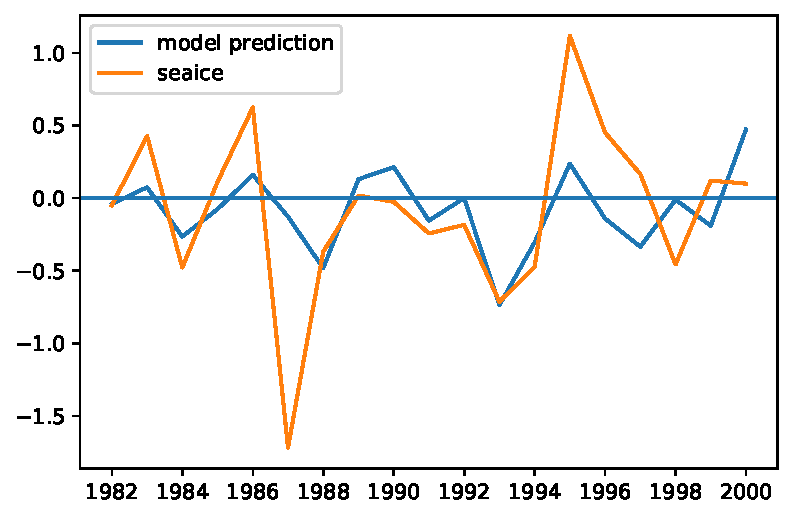
\includegraphics{Images_3.0/regressions/multivariate_model_anomalous_n1_annually_detrended_1979_2000.pdf}
    \caption{Fitted model for SIE detrended and averaged annually from 1979 to 2000.}
    \label{fig:multivariate_model_anomalous_n1_annually_detrended_1979_2000}
    \end{subfigure}
    
    \begin{subfigure}{\linewidth}
    \centering
    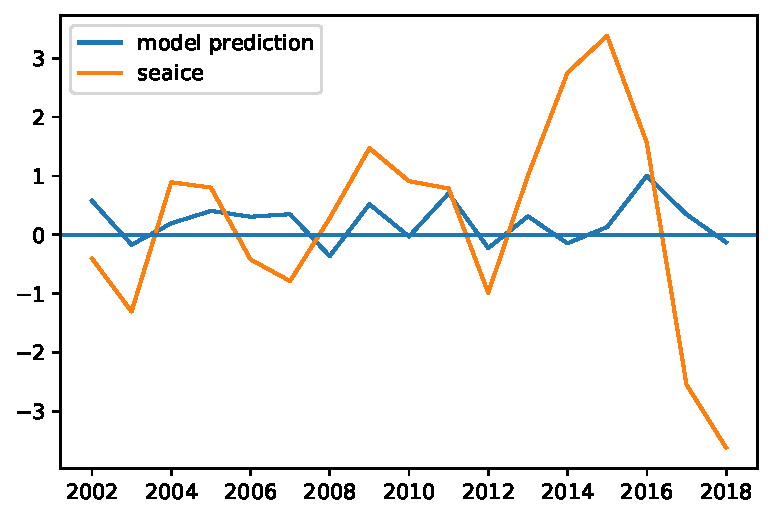
\includegraphics{Images_3.0/regressions/multivariate_model_anomalous_n1_annually_detrended_2001_2018.pdf}
    \caption{Fitted model for SIE detrended and averaged annually from 2001 to 2018.}
    \label{fig:multivariate_model_anomalous_n1_annually_detrended_2001_2018}
    \end{subfigure}
    \caption{Fitted model for SIE detrended and averaged annually. Before and after December 2000.}
\end{figure}

Likewise to looking at the entire time period, these plots are also demonstrating a bad fitting \textcolor{red}{put these in the same plot for easier comparison?}. For the same reasons as before this is unsurprising.

\newpage
\section{Spatial Regressions}
Looking at the regression analysis with the mean SIE we note that most of our fittings are not of great quality or statistically significant. We hope by introducing a spatial component to our analysis we can produce better quality results and begin to develop a more physical understanding of how these circulations impact the variability of sea ice in Antarctica.
Like before we start by doing individual regressions with each index we are interested in.
\begin{figure}[H]
    \centering
    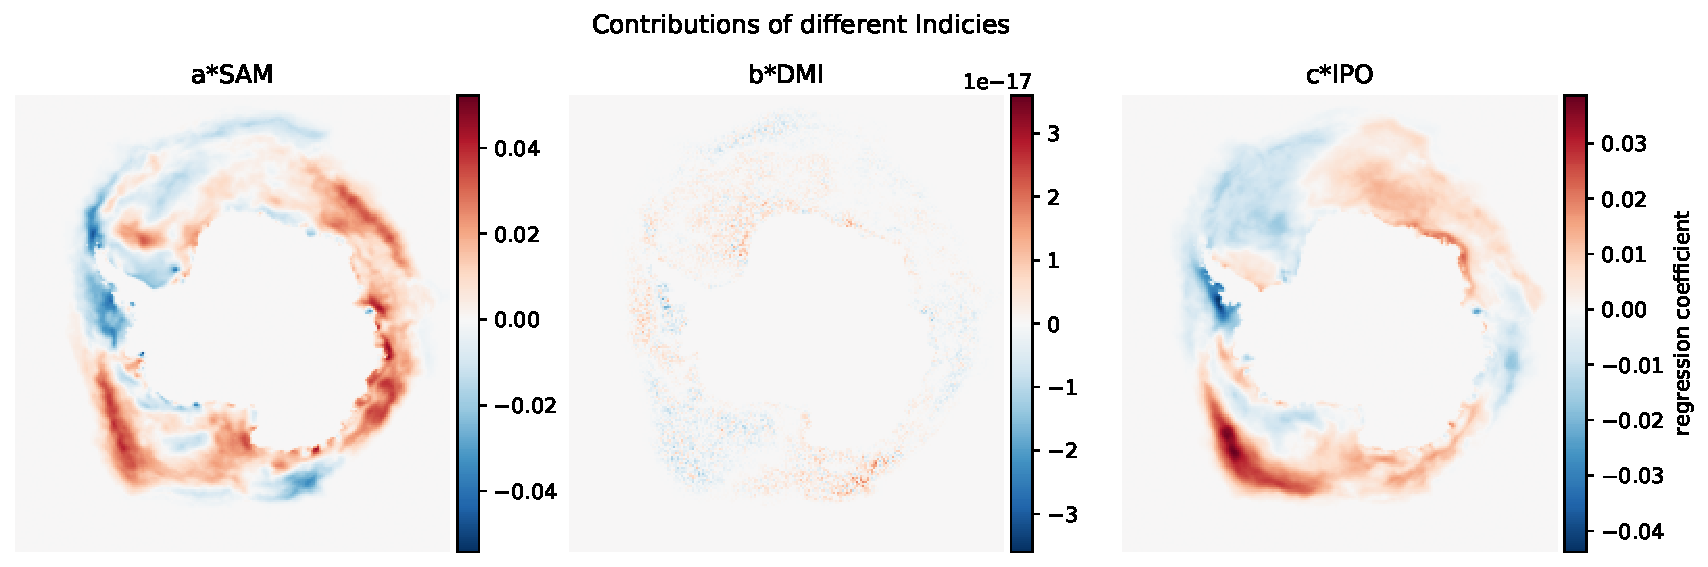
\includegraphics[width=\linewidth]{Images_3.0/regressions/index_contribution_anomalous_n1_annually_1979_2018.pdf}
    \caption[Spatial distribution of regression of SIC for each of the indices for 1979 to 2018]{Spatial distribution of regression of SIC for each of the indices for 1979 to 2018. Blue indicates a negative contribution and red indicates a positive contribution.}
    \label{fig:index_contribution_anomalous_n1_annually_1979_2018}
\end{figure}
Looking at these plots there are two main things which are notable. The first is that the expected contribution by DMI is much lower than the other two circulation patterns. For SAM this makes sense as it is localised around Antarctica. For IPO it also makes sense as the circulation is based over the Pacific \textcolor{red}{link this to the literature review.} The other thing to note is that the contribution of SAM and IPO are spatially very similar. This is interesting as we hypothesised that they impact the sea ice in Antarctica in different ways. It looking like SAM was more impactful for long term trends and IPO was more impactful for short term variability. This may or may not be the case. To understand this further we will need to look at the literature. As before this is done with a linear fitting, as such we don't expect the patterns here to indicate more that the base relationship that exists between these circulations and the behaviour of Sea ice in and around Antarctica. Likewise to before we will perform this same analysis, splitting the time series at the end of 2000, when IPO is noted to change it's overall phase. This can be seen below.

\begin{figure}[H]
    \begin{subfigure}{\linewidth}
    \centering
    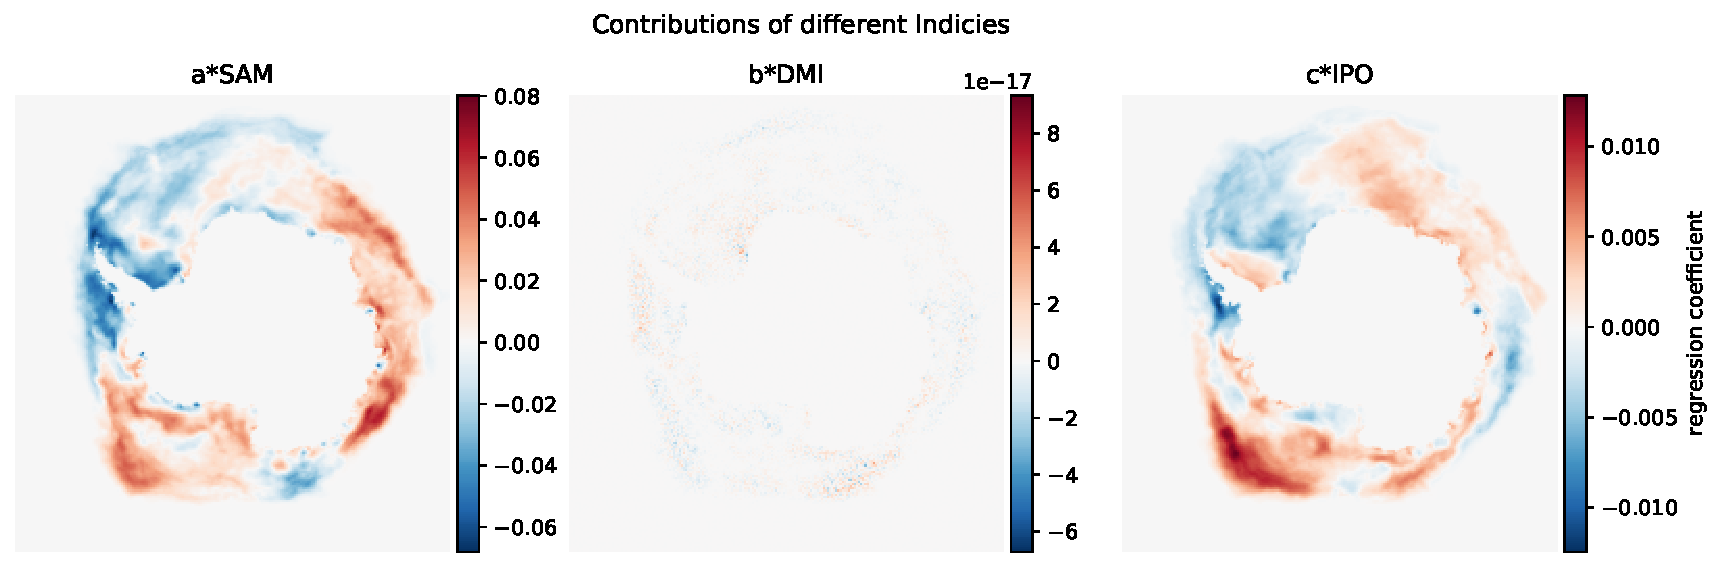
\includegraphics[width=\linewidth]{Images_3.0/regressions/index_contribution_anomalous_n1_annually_1979_2000.pdf}
    \caption{Spatial distribution of regression of SIC for each of the indices for 1979 to 2000.}
    \label{fig:index_contribution_anomalous_n1_annually_1979_2000}
    \end{subfigure}
    
    \begin{subfigure}{\linewidth}
    \centering
    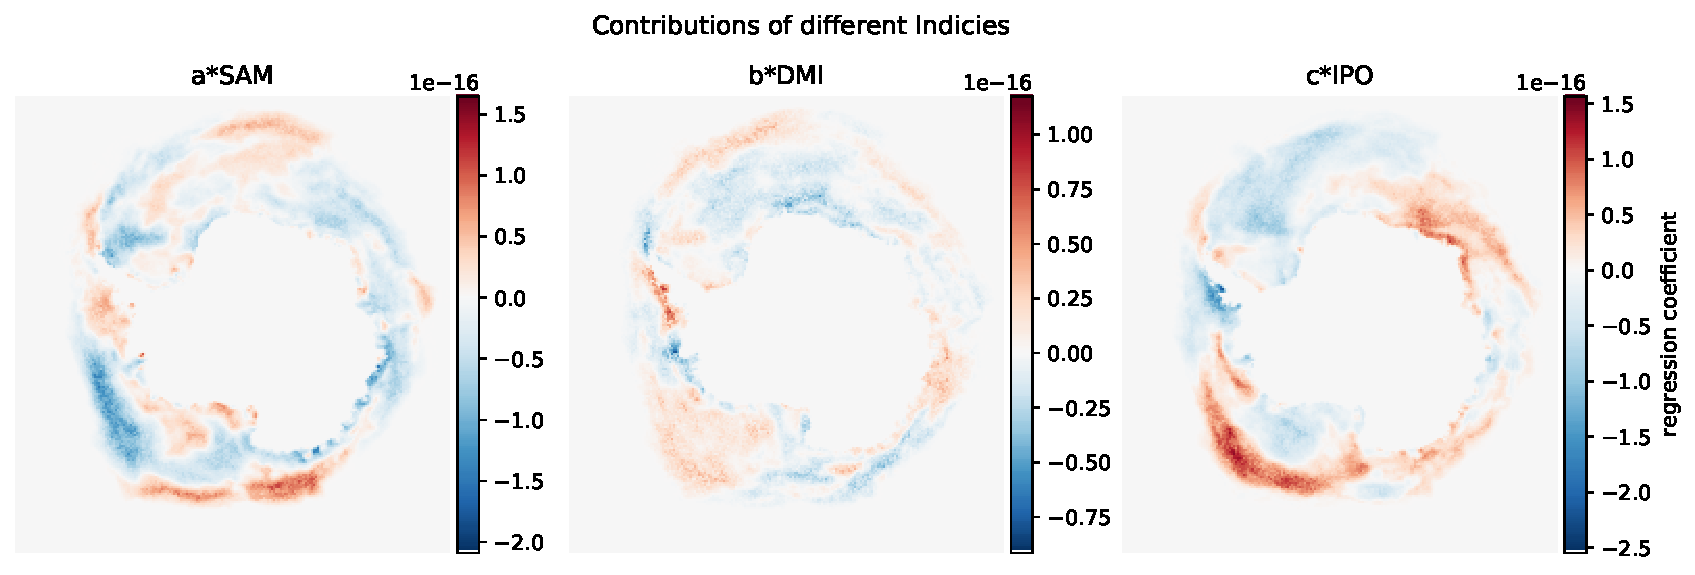
\includegraphics[width=\linewidth]{Images_3.0/regressions/index_contribution_anomalous_n1_annually_2001_2018.pdf}
    \caption{Spatial distribution of regression of SIC for each of the indices for 2001 to 2018.}
    \label{fig:index_contribution_anomalous_n1_annually_2001_2018}
    \end{subfigure}
    \caption{Spatial distribution of regressions for SIE for the different time periods in our dataset.}
\end{figure}